\section{Structural members selection procedure}

To start the structural members selection, it is needed to be known the longest dimensions of each member. It can be achieved by implementing an algorithm which compares all the dimensions of each module. All of this information has been stored in a Python dictionary.

\subsection{Load study}

As defined on AISI S100-16 standard, load distribution can be segmented in \textit{dead}, \textit{live}, \textit{product} and \textit{combined} loads. 

\subsubsection{Dead load}

It consists of the weight of the structural members. It depends on the densisty of the material, the cross sectional area and the length of the member.

\begin{equation}
    D = A \rho L g
    \label{eq:dead}
\end{equation}

From Equation $\eqref{eq:dead}$, $D$ correspond to the value of the dead load, $A$ to the cross sectional area, $L$ to the length of the member and $g$ to gravity's acceleration.

\subsubsection{Live load}

The distirbuted live load for the food traffic on pick module walkways should be, at least, of $293 \left[kg / m^2 \right]$, according to the standard ANSI MH16, section 8.4.2. The live load can be calculated using Equation. $\eqref{eq:live}$.

\begin{equation}
    L = L_{dist} A g
    \label{eq:live}
\end{equation}

 Where: $L$ is the live load, $L_{dist}$ is the distributed load, $A$ correspond to the area of the biggest module and $g$ to the gravity.

\subsubsection{Product load}

The product load correspond to the difference between the design distributed load, the live load and the dead load.

\subsubsection{Combined load}

The combined load is used to determine the stresses of the structural members. There was used a Load and Resistance Factor Design (LRFD, ANSI MH16.1 section 2.1) as seen on Equation $\eqref{eq:combinedload}$.

\begin{equation}
    CL = 1.2 D + 1.4 P +1.6 L
    \label{eq:combinedload}
\end{equation}

Where: $CL$ is the combined load, $D$ is the dead load (Eq. $\eqref{eq:dead}$), $P$ is the product load and $L$ is the live load (Equation $\eqref{eq:live}$).

\subsection{Joists}

Structural design of joists is evaluated based on the maximum momentum compared \textit{nominal resistance momentum} (section 3.3.2.2.2 of AISI S100-16 standard).

\begin{figure}[h!]
\centering
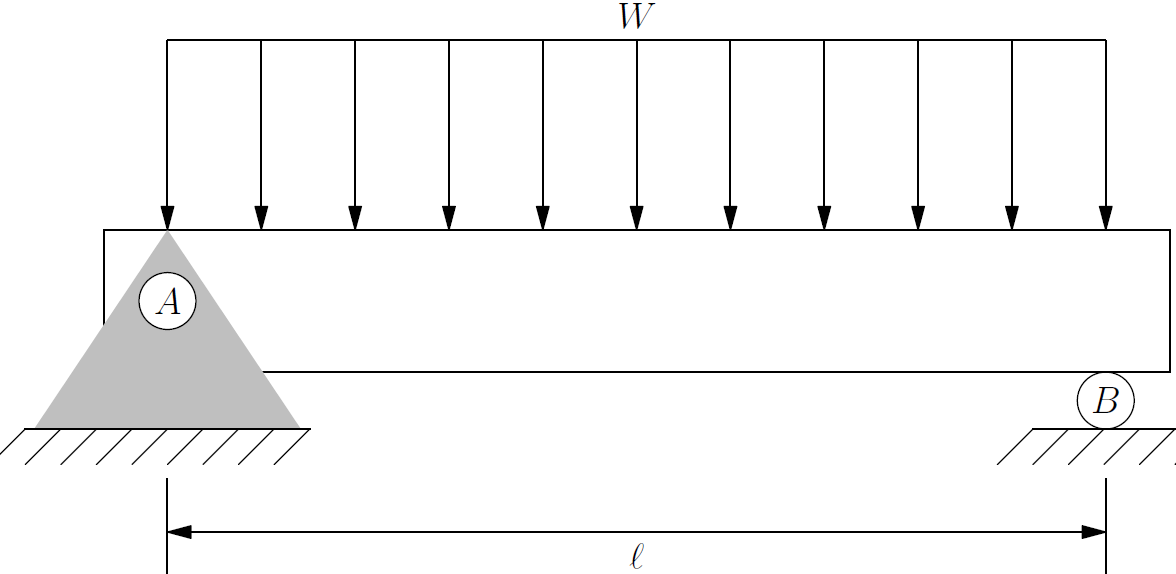
\includegraphics[width=\textwidth]{Images/Calculus/Vigueta/Vigueta.PNG}
\caption{Load distribution over a joist.}
\label{distjoist}
\end{figure}

As it can be appreciated on Figure \ref{distjoist}, the calculation proccess starts by the supposition of a simply supported beam. The distributed load $W$ correspond to the combined load, from Equation $\eqref{eq:combinedload}$. The momentum behaviour over the joist is defined by Equation $\eqref{eq:joistmoment}$.

\begin{equation}
M(x) = \frac{W x (L-x)}{2}
\label{eq:joistmoment}
\end{equation}

According to the Equation $\eqref{eq:joistmoment}$, the maximum momentum is:

\begin{equation}
M = \frac{W L^2}{8}
\end{equation}

\subsubsection{Selection}

Joist selection is developed by each of the structural profile in the database. For each of them is evaluated and compared both maximum momentum and nominal resistance momentum. The final selection is to the member with the lowest cross sectional area, for this example the summary table is shown on Figure \ref{joistselec}.

\begin{figure}[h!]
\centering
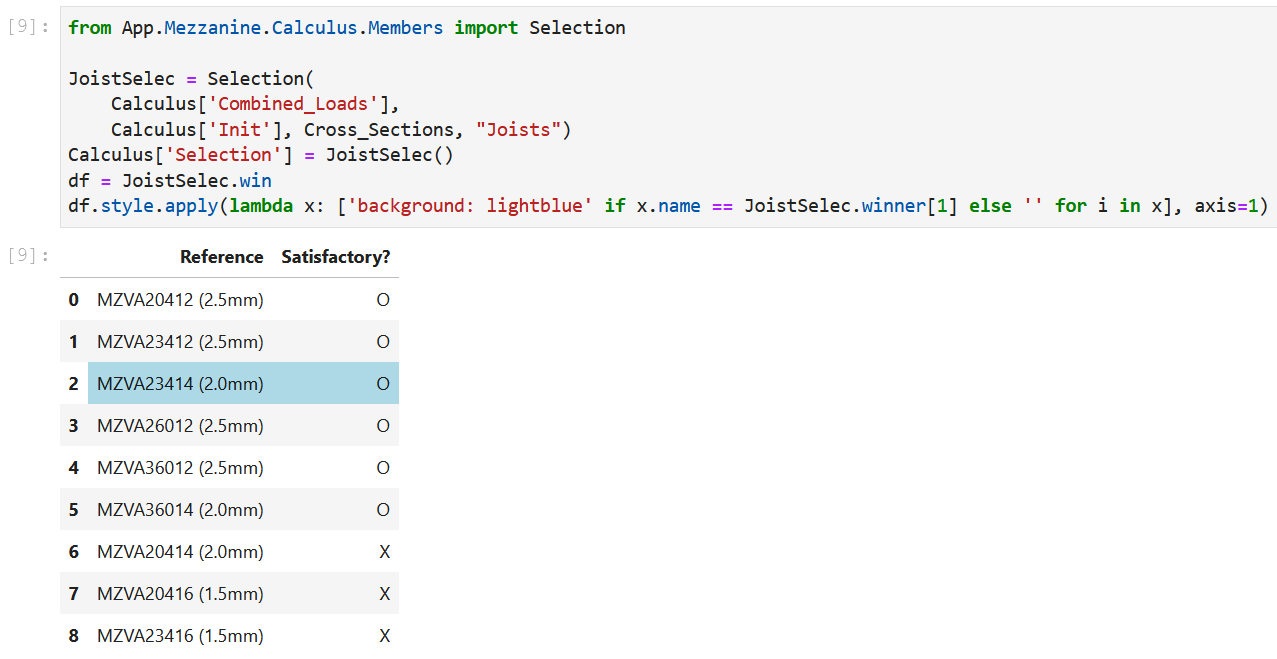
\includegraphics[width=\textwidth]{Images/Calculus/viguetaselec.PNG}
\caption{Selection table.}
\label{joistselec}
\end{figure} 

From Table \ref{joistselec}, the selected member is `MZVA23414 (2.0 mm)'.

\subsection{Beams}

The structural evaluation procedure is the same as joists (section 3.2).

\begin{figure}[h!]
\centering
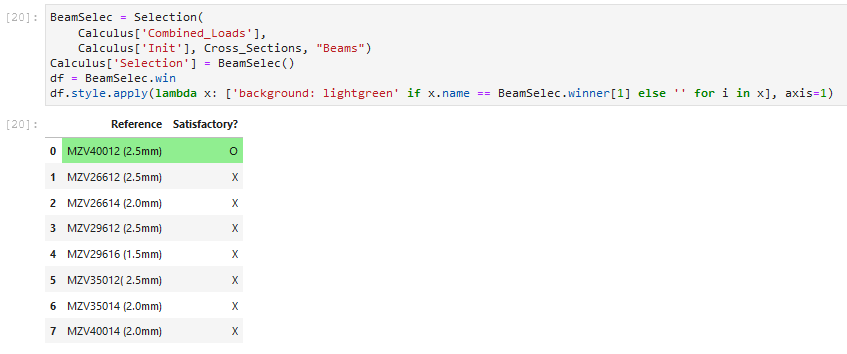
\includegraphics[width=\textwidth]{Images/Calculus/vigaselec.PNG}
\caption{Selection table for beams.}
\label{beamselec}
\end{figure} 

\subsection{Columns}

Unlike beams and joists, columns are multiaxial load members. When the column of a structure fails it is mainly because of flexural-torsional buckling stresses (`large' columns) or axial stresses (`short' columns). The procedure starts by evaluating compression load (axial stress) and compare it with the nominal load (result of the defined procedure given by the AISI S100-16 standard)  for each option of the database. If the nominal load has a bigger value than the calculated compression load, then it can be concluded that axial stress is not critical so the momentum due to flexural-torsional buckling should be compared with nominal momentum (defined by AISI S100-16 standard) to discard failure by buckling stresses. The results for the given example is shown on Figure \ref{column}.

\begin{figure}[h!]
\centering
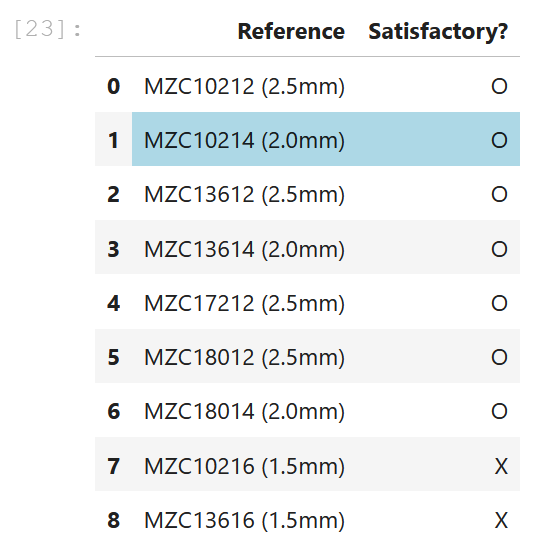
\includegraphics[width=\textwidth]{Images/Calculus/columnselec.PNG}
\caption{Column selection table.}
\label{columnselec}
\end{figure}

From Figure \ref{columnselec}, the column of reference `MZC10214' has been selected.